\documentclass{article}
\usepackage{amsmath}
\usepackage{amssymb}
\usepackage{graphicx}
\usepackage{hyperref}
\usepackage[version=4]{mhchem}

\title{Problem 6}
\date{}

\begin{document}
\maketitle

\section*{Problem}
\(A B=2 R\) is the diameter of the semicircle as shown in the figure. Two circles \(P\left(r_{1}\right)\) and \(Q\left(r_{2}\right)\) inscribed in the semicircle and are tangent to each other and to \(A B\) at \(O\) and \(K\), respectively. Find the length of \(r_{2}\).\\
\centering
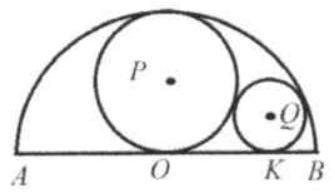
\includegraphics[width=\textwidth]{images/problem_image_1.jpg}

\section*{Solution}
Connect \(O P, K Q, P Q\). Draw \(Q N / / A B\) to meet \(P O\) at \(N\).\\
\(P O=\frac{1}{2} R, P Q=\frac{1}{2} R+r_{2}\),\\
\centering
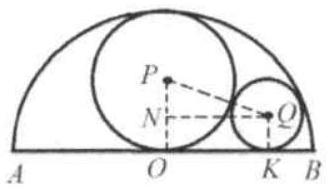
\includegraphics[width=\textwidth]{images/reasoning_image_1.jpg}

Applying Pythagorean Theorem to \(\triangle P O N\) :\\
\(O K^{2}=P Q^{2}-P N^{2}\)


\(=\left(\frac{1}{2} R+r_{2}\right)^{2}-(P O-N O)^{2}\)\\
\(=\left(\frac{1}{2} R+r_{2}\right)^{2}-\left(\frac{1}{2} R-r_{2}\right)^{2}\)\\
\(=2 R r_{2}\).\\
So \(O K=\sqrt{2 R r_{2}}\).\\
We also know that \(\frac{1}{A K}+\frac{1}{K B}=\frac{1}{Q K} \Rightarrow \frac{1}{R+\sqrt{2 R r_{2}}}+\frac{1}{R-\sqrt{2 R r_{2}}}=\frac{1}{r_{2}}\)\\
\(\Rightarrow \quad r_{2}=\frac{1}{4} R\).

\end{document}
